\documentclass[11pt]{article}

\RequirePackage[colorlinks]{hyperref}

\usepackage{amsmath}
\usepackage{amsthm}
\usepackage{amssymb}
\usepackage{verbatim}
\usepackage{url}
\usepackage{fullpage}
\usepackage{graphicx}
\usepackage{enumerate}
\usepackage[usenames,dvipsnames]{xcolor}
\usepackage{graphicx}




\begin{document}


\begin{center}
\textbf{\textcolor{Blue}{New York University Shanghai}} \\
~~\\
\textbf{\Large Problem Set 1}
\\
~
\\
\textbf{\small BUSF-SHU 210: Business Analytics (Spring 2018)} \\
~~\\\textbf{Due at 10:00PM on Sunday, Feb 11}
\end{center}
\noindent\textbf{Instructions}
\\
~
\\
Whenever you are asked to build a linear regression model, you should write out the model in the form of
$$Y_i\approx\beta_0+\sum_{j=1}^p\beta_j X_{ij},$$
and clearly explain what are the variables $Y_i$, $X_{i1}$, $X_{i2}$, $\dots$, $X_{ip}$. After running the model to get the estimated values of $\hat{\beta}_0$, $\hat{\beta}_1$, $\dots$, $\hat{\beta}_p$, please report the results in the form of
$$Y_i\approx\hat{\beta}_0+\sum_{j=1}^p\hat{\beta}_j X_{ij},$$
and interpret what the coefficients $\hat{\beta}_0$, $\hat{\beta}_1$, $\dots$, $\hat{\beta}_p$ mean in the problem of interest. %You should also report
\\
~
\\
\noindent\textbf{1. Greenhouse Effect}
\\
~
\\
You will attempt to study the relationship between average global temperature and several other factors.
The file \verb+greenhouse.csv+ contains the climate data from 1983 to 2008. The variables are listed as follows:
\begin{itemize}
\item $Year$: the observation year.

\item $Month$: the observation month.
\item $Temp$: the difference between the average global temperature and a reference value in that month.
\item $CO2$, $N2O$, $CH4$, $CFC.11$, $CFC.12$: concentrations of carbon dioxide (CO2), nitrous oxide (N2O), methane  (CH4), trichlorofluoromethane (CCl3F; commonly referred to as CFC-11) and dichlorodifluoromethane (CCl2F2; commonly referred to as CFC-12), respectively, in the atmosphere. $CO2$, $N2O$ and $CH4$ are expressed in ppmv (parts per million by volume, i.e., 397 ppmv of CO2 means that CO2 constitutes 397 millionths of the total volume of the atmosphere)

\item $CFC.11$ and $CFC.12$ are expressed in ppbv (parts per billion by volume).
\item $Aerosols$: the mean stratospheric aerosol optical depth at 550 nm. This variable is linked to volcanoes.

\item $TSI$: the total solar irradiance (TSI) in $W/m^2$ (the rate at which the sun's energy is deposited per unit area).

\item	$MEI$: multivariate El Nino Southern Oscillation index (MEI), a measure of the strength of the El Nino/La Nina-Southern Oscillation.

\end{itemize}
~
\\
(a) Read the dataset \verb+greenhouse.csv+ into $R$. Then, split the data into a training set, consisting of all the observations up to and including 2005, and a testing set consisting of the remaining years. A training set is the data that will be used to build the model, and a testing set is the data to test the predictive ability.
\\
~
\\
Build a linear regression model to establish the association between the dependent variable $Temp$, and the independent variables $MEI$, $CO2$, $CH4$, $N2O$, $CFC.11$, $CFC.12$, $TSI$, and $Aerosols$. Use the training set to build the model.
\\
~
\\
Please show a screen shot of your linear regression model using the ``summary" function and interpret the results. Clearly state the significance, the sign, and the magnitude of the association between the dependent variable and each independent variable. Figure \ref{fig:q1}
\begin{figure}[htbp]
  \centering
  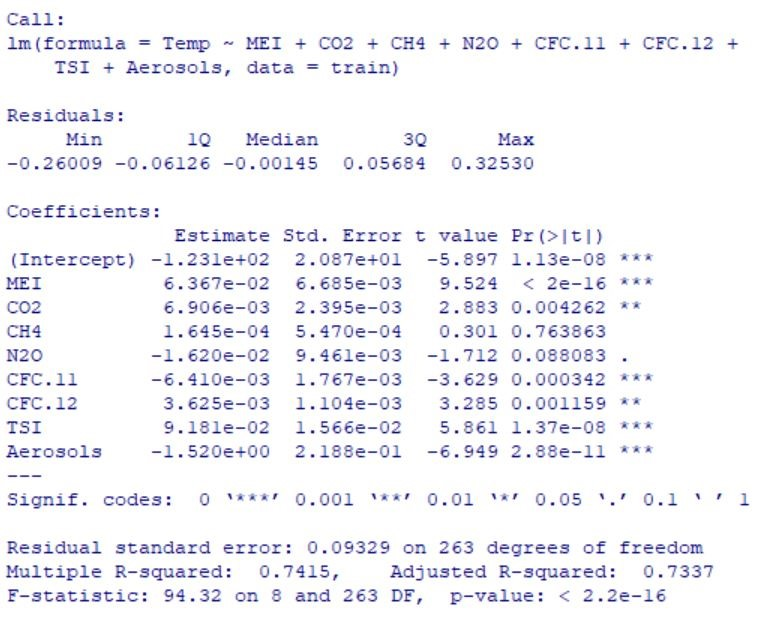
\includegraphics[width=0.4\textheight]{1a.jpg}
  \caption{Question 1(a)}\label{fig:q1}
\end{figure}

\textcolor{Blue}{Temp = -123.1 + 0.06367*MEI + 0.006906 * CO2 + 0.0001645 * CH4 - 0.01620 * N2O �C 0.00641 * CFC.11 + 0.003625 * CFC.12 + 0.09181 * TSI -1.52 * Aerosols}
\\
\textcolor{Blue}{
\begin{itemize}
\item	$MEI$ : significant, positive, one unit change in MEI is associate with 0.064 increase in Temp
\item	$CO2$ : significant, positive, one unit change in CO2 is associate with 0.007 increase in Temp
\item	$CH4$ : insignificant, positive, one unit change in CH4 is associate with 0.0002 increase in Temp
\item	$N2O$ : insignificant, negative, one unit change in NO2 is associate with 0.016 decrease in Temp
\item	$CFC.11$ : significant, negative, one unit change in CFC.11 is associate with 0.006 decrease in Temp
\item	$CFC.12$ : significant, positive, one unit change in CFC.12 is associate with 0.004 increase in Temp
\item	$TSI$ : significant, positive, one unit change in TSI is associate with 0.092 increase in Temp
\item	$Aerosols$ : significant, negative, one unit change in Aerosols is associate with 1.520 decrease in Temp
\end{itemize}}
~
\\


(b) It is widely believed that nitrous oxide and CFC-11 are greenhouse gases. From the regression analysis in part (a), is there anything counter-intuitive about the regression results? Please provide some explanation supported by quantitative evidence for such counter-intuitive phenomenon. (\textit{Hint}: You may want to check the correlations between different independent variables.)
\\
\\
\textcolor{Blue}{In the regression model, the coefficients for N2O and CFC.11 are negative, meaning that the higher N2O and CFC.11 are, the lower the temperature is, which is counter-intuitive. In addition, if we use p value to determine significance, N2O is not that significant while it actually is a greenhouse gas. Both problems are due to the multicollinearity between the selected variables.}  Figure \ref{fig:q1.2}
\\
\begin{figure}[htbp]
  \centering
  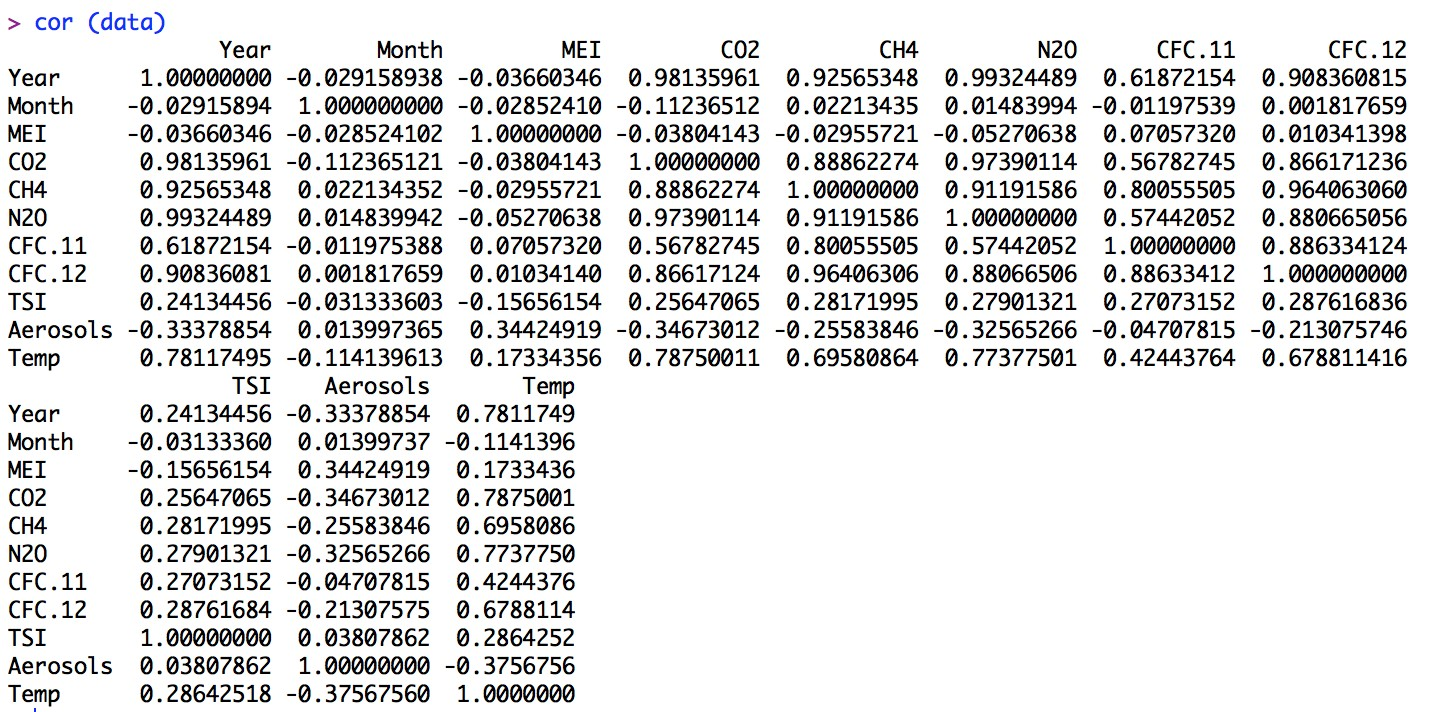
\includegraphics[width=0.4\textheight]{1b.jpg}
  \caption{Question 1(b)}\label{fig:q1.2}
\end{figure}
~
\\
~
\textcolor{Blue}{Here we regard correlation as high if the absolute value of correlation $>$ 0.7, so N2O is highly correlated with CO2, CH4 and CFC.12; CFC.11 is highly correlated with CH4 and CFC.12.}
\\
~
\\
\\
(c) Based on your analysis of parts (a) and (b), build another (possibly simpler with fewer covariates) linear regression model. Test both the full model (i.e., the one developed in part (a)) and the new model using the testing data. Report the respective out-of-sample $R^2$'s for both models. Which one performs better?
\\

\textcolor{Blue}{Since there are strong correlation among the variables N2O, CO2, CH4, CFC.11 and CFC.12, we would only select one of the above variables. The new regression model (see Figure \ref{fig:q1.3} ) is as follows:}
\\
\\
\textcolor{Blue}{Temp = - 109.8 + 0.0638 * MEI + 0.02608 * N2O + 0.07462 * TSI -1.681 * Aerosols}
\\
\\
\begin{figure}[htbp]
  \centering
  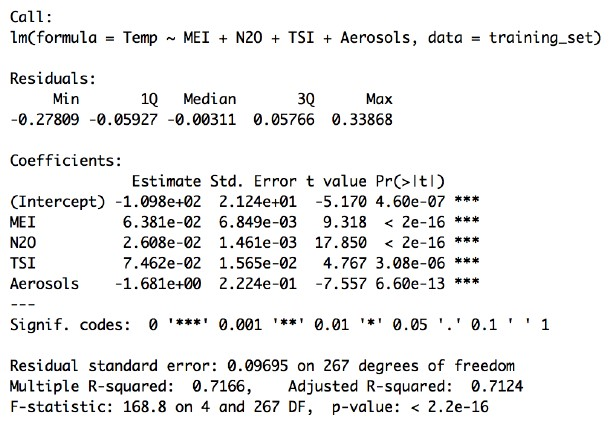
\includegraphics[width=0.4\textheight]{1c.jpg}
  \caption{Question 1(c)}\label{fig:q1.3}
\end{figure}
~
\\
\textcolor{Blue}{
Out-of-sample R-squared for model 1 = 0.7631
\\
Out-of-sample R-squared for model 2 = 0.6582
\\
Model 1 performs better, partly because model 2 loses quite a lot information by eliminating 4 variables.
}
~
\\

\newpage
\noindent\textbf{2. Student Assessment Scores}
\\
~
\\
In this problem, you will predict the reading scores of students on the 2009 Assessment.
\\
~
\\
The datasets \verb+Assessment_train.csv+ and \verb+Assessment_test.csv+ contain information about the students taking the exam.
\\~\\
Each row in the datasets \verb+Assessment_train.csv+ and \verb+Assessment_test.csv+ represents one student taking the Assessment. The datasets have the following variables:
\begin{itemize}
\item $grade$: The grade in school of the student (most 15-year-olds in America are in 10th grade)
\item $male$: Whether the student is male (1/0)
\item $raceeth$: The race/ethnicity composite of the student
\item $preschool$: Whether the student attended preschool (1/0)
\item $expectBachelors$: Whether the student expects to obtain a bachelor's degree (1/0)
\item $motherHS$: Whether the student's mother completed high school (1/0)
\item $motherBachelors$: Whether the student's mother obtained a bachelor's degree (1/0)
\item $motherWork$: Whether the student's mother has part-time or full-time work (1/0)
\item $fatherHS$: Whether the student's father completed high school (1/0)
\item $fatherBachelors$: Whether the student's father obtained a bachelor's degree (1/0)
\item $fatherWork$: Whether the student's father has part-time or full-time work (1/0)
\item $selfBornUS$: Whether the student was born in the United States of America (1/0)
\item $motherBornUS$: Whether the student's mother was born in the United States of America (1/0)
\item $fatherBornUS$: Whether the student's father was born in the United States of America (1/0)
\item $englishAtHome$: Whether the student speaks English at home (1/0)
\item $computerForSchoolwork$: Whether the student has access to a computer for schoolwork (1/0)
\item $read30MinsADay$: Whether the student reads for pleasure for 30 minutes/day (1/0)
\item $minutesPerWeekEnglish$: The number of minutes per week the student spend in English class
\item $studentsInEnglish$: The number of students in this student's English class at school
\item $schoolHasLibrary$: Whether this student's school has a library (1/0)
\item $publicSchool$: Whether this student attends a public school (1/0)
\item $urban$: Whether this student's school is in an urban area (1/0)
\item $schoolSize$: The number of students in this student's school
\item $readingScore$: The student's reading score, on a 1000-point scale
\end{itemize}
\noindent There are some missing values in this data set, which we need to remove before building the linear regression model. Use the function \verb+na.omit()+ to remove the missing values in both the training data and the testing data. To apply this function, you may type: \verb+AssesmentTrain = na.omit(AssessmentTrain)+ and \verb+Assessment = na.omit(AssessmentTest)+ in the R console.
\\
~
\\
(a) Factor variables are variables that take on a discrete set of values, like the ``Region" variable in the WHO data set from the exercises of Session 1.An ordered factor has a natural ordering between the levels (an example would be the classifications ``large," ``medium," and ``small"). Which of the variables in the Assessment data set are unordered factors with at least three levels? Which of the variables are ordered factors with at least three levels?
\\
\\
\textcolor{Blue}{ From summary(AssessmentTrain), we can see that raceeth is the unordered factor with at least three levels, and grade is the ordered factor with at least three levels. (minutesPerWeekEnglish, studentsInEnglish, schoolSize, and readingscore could be counted as ordered factors as well)}
~
\\
\\
(b) To include unordered factors in a linear regression model, we define one level as the ``reference level" and add a binary variable for each of the remaining levels. In this way, a factor with $n$ levels is replaced by $n-1$ binary variables. The reference level is typically selected to be the most frequently occurring level in the dataset.
\\
~
\\
As an example, consider the unordered factor variable ``place", with levels ``Shanghai", ``Beijing", and ``Guangzhou". If ``Beijing" were the reference level, then we would add binary variables ``placeShanghai" and ``placeGuangzhou" to a linear regression problem. All Shanghai examples would have placeShanghai=1 and placeGuangzhou=0. All Guangzhou examples would have placeShanghai=0 and placeGuangzhou=1. All Beijing examples would have placeShanghai=0 and placeGuangzhou=0.
\\
~
\\
Now, consider the variable ``raceeth" in our problem, which has levels ``American Indian/Alaska Native", ``Asian", ``Black", ``Hispanic", ``More than one race", ``Native Hawaiian/Other Pacific Islander", and ``White". Because it is the most common in the data set, we will select White as the reference level. Which binary variables should be included in the regression model? For a student who is Asian, which of the binary variables you created above should be set to 0, which of them should be set to 1?
\\
\\
\textcolor{Blue}{��raceethAmerican Indian/Alaska Native", ��raceethAsian", ��raceethBlack", ��raceethHispanic", ��raceethMore than one race", and ��raceethNative Hawaiian/Other Pacific Islander�� should be included.
\\
For a student who is Asian, ��raceethAsian" should be set to 1; All other binary variables,  ��raceethAmerican Indian/Alaska Native",  ��raceethBlack", ��raceethHispanic", ��raceethMore than one race", and ��raceethNative Hawaiian/Other Pacific Islander�� should be set to 0.}
\\
~
\\
(c) Because the race variable takes on text values, by default $R$ selects the first level alphabetically (``American Indian/Alaska Native") as the reference level, instead of the most common level (``White"). To reset the reference level of the factor, we can use the following two commands in the R console: \verb+AssessmentTrain$raceeth = relevel(AssessmentTrain$raceeth, "White")+ and
\verb+AssessmentTest$raceeth = relevel(AssessmentTest$raceeth, "White")+. Build a linear regression model to predict the reading score of students using all remaining variables as covariates. Use the training set to build the model.
\\
~
\\Please show a screen shot of your linear regression model using the ``summary" function. Find the independent variables that are significant (with $p-$value, $Pr(>|t|)$, smaller than 0.05). Consider two students A and B. They have all variable values the same, except that student A is in grade 11 and student B is in grade 9. What is the predicted reading score of student A minus the predicted reading score of student B? Please interpret the estimated coefficient of the variable ``Asian''. Figure \ref{fig:q2}
\\
\\
\textcolor{Blue}{readingScore = 143.77 + 29.54 * grade -14.52*male -67.28 * raceethAmerican Indian/Alaska Native -4.11*raceethAsian -67.01*raceethBlack -38.98*raceethHispanic -16.92 * raceethMore than one race - 5.10 * raceethNative Hawaiian/Other Pacific Islander - 4.46 * preschool + 55.27 * expectBachelors + 6.05 * mothers + 12.64 * motherBachelors -2.81 * motherWork + 4.02 * fathers + 16.93 * fatherBachelors + 5.84 * fatherWork -3.81 * selfBornUS - 8.80 * motherBornUS + 4.31 * fatherBornUS +8.04 * englishAtHome + 22.50 * computerForSchoolwork + 34.87 * read30MinsADay +0.01 * minutesPerWeekEnglish + 12.22 * schoolHasLibrary -16.86 * publicSchool -0.11* urban +0.01 * schoolSize
\\
\\
\begin{itemize}
\item	$raceethAmerican Indian/Alaska Native$ : one unit change in raceethAmerican Indian/Alaska Native is associate with 67.28 decrease in readingScore
\item	$raceethAsian$ : one unit change in raceethAsian is associate with 4.11 decrease in readingScore
\item	$raceethBlack$ : one unit change in raceethBlack is associate with 67.01 decrease in readingScore
\item	$raceethHispanic$ : one unit change in raceethHispanic is associate with 38.98 decrease in readingScore
\item	$raceethMore than one race$ : one unit change in raceethMore than one race is associate with 16.92 decrease in readingScore
\item	$raceethNative Hawaiian/Other Pacific Islander$ : one unit change in raceethNative Hawaiian/Other Pacific Islander is associate with 5.10 decrease in readingScore
\end{itemize}}
~
\\
\\\begin{figure}[htbp]
  \centering
  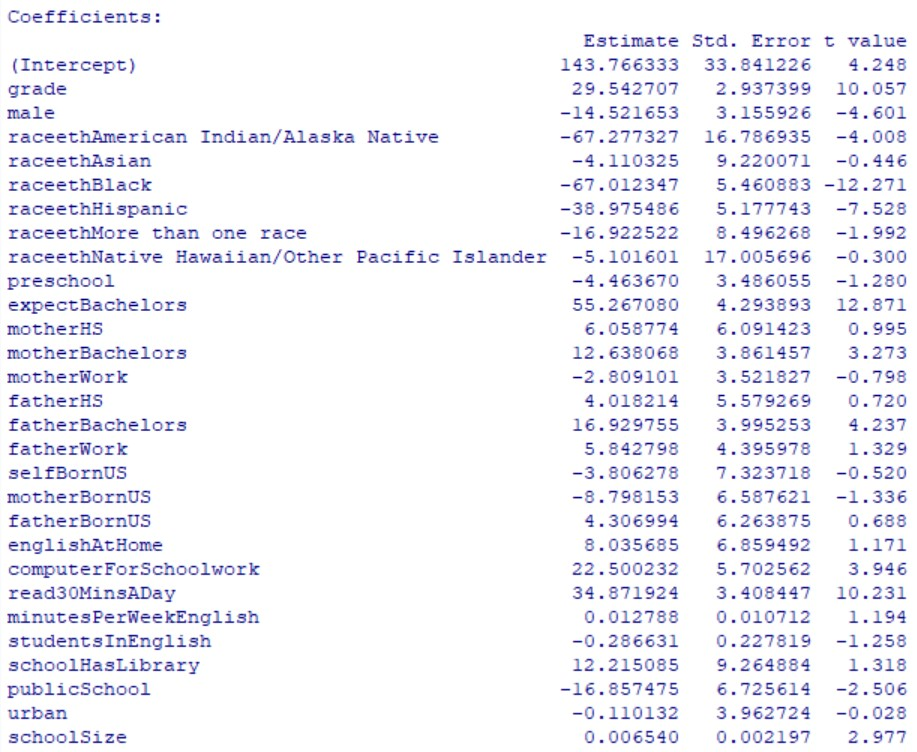
\includegraphics[width=0.4\textheight]{2c1.jpg}
\end{figure}
\\
\\
\\\begin{figure}[htbp]
  \centering
  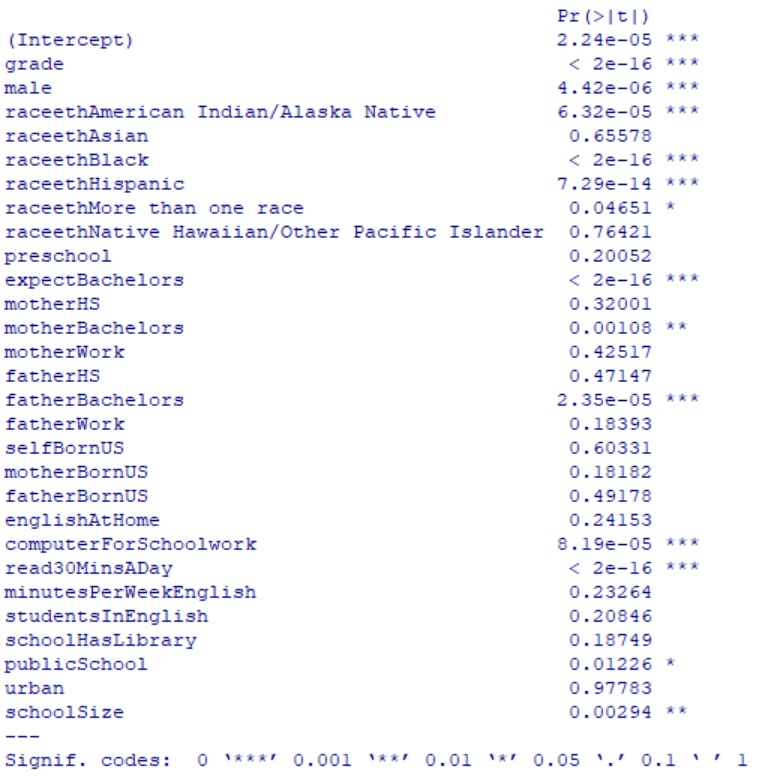
\includegraphics[width=0.4\textheight]{2c2.jpg}
  \caption{Question 2(c)}\label{fig:q2}
\end{figure}
~
\\
\\
\textcolor{Blue}{Significant variables: grade, male, raceeth, expectBachelors, motherBachelors, fatherBachelors, computerForeSchoolwork, read30MinsADay, publicSchool, and schoolSize.
\\
\\
Predicted score difference between student A and B is 29.54*2 = 59.08.
\\
\\
The estimated coefficient of the variable raceethAsian equals -4.11, meaning that, if all else equal, Asian students are estimated to have reading scores 4.11 points lower than the white students.}
\\
\\
(d) If we remove all the independent variables that are not significant (with $p-$value, $Pr(>|t|)$, no smaller than 0.05), we can build a new linear regression model. Test both the full model (i.e., with all the variables in the data set as independent variables) and the new model (i.e., with the insignificant variables removed) using the testing data. Report the respective out-of-sample $R^2$'s for both models.
\\
\\
\textcolor{Blue}{The out-of-sample R-squared for the full model is 0.2615.
\\
The out-of-sample R-squared for the simplified model is 0.2657.}

\newpage
\noindent\textbf{3. Forecasting Auto Sales}
\\
~
\\
In this problem, we will try to predict monthly sales of an Auto Brand.
\\
~
\\The file \verb+Auto.csv+ contains data for the problem. Each observation is a month, from January 2010 to February 2014. For each month, we have the following variables:
\begin{itemize}
\item	$Month$ = the month of the year for the observation (1 = January, 2 = February, 3 = March, ...).
\item	$Year$ = the year of the observation.
\item	$AutoSales$ = the number of units of the Auto sold in the United States in the given month.
\item	$Unemployment$ = the estimated unemployment percentage in the United States in the given month.
\item	$Queries$ = a (normalized) approximation of the number of Google searches for ``Auto" in the given month.
\item	$CPI\_energy$ = the monthly consumer price index (CPI) for energy for the given month.
\item	$CPI\_all$ = the consumer price index (CPI) for all products for the given month; this is a measure of the magnitude of the prices paid by consumer households for goods and services (e.g., food, clothing, electricity, etc.).
\end{itemize}
\noindent Load the data set into $R$ and split the data set into training and testing sets as follows: Place all observations for 2012 and earlier in the training set, and all observations for 2013 and 2014 into the testing set.
\\
~
\\
(a) Build a linear regression model to predict monthly Auto sales using Unemployment, CPI\_all, CPI\_energy and Queries as the independent variables. Use all of the training set data to do this. Please show a screen shot of your linear regression model using the ``summary" function. Clearly state the significance, the sign, and the magnitude of the association between the dependent variable and each independent variable. Figure \ref{fig:q3}
\\

\begin{figure}[htbp]
  \centering
  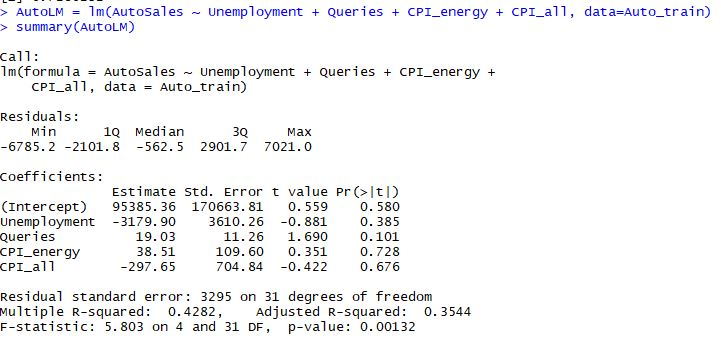
\includegraphics[width=0.6\textheight]{3a.jpg}
  \caption{Question 3(a)}\label{fig:q3}
\end{figure}



~
\\
\textcolor{Blue}{AutoSales = 95385.36 -3179.90Unemployment + 19.03Queries + 38.51CPI\_energy -297.65CPI\_all
\\
\begin{itemize}
\item	$Unemployment$ : insignificant, negative, one unit change in Unemployment is associate with 3179.90 decrease in Auto Sales
\item	$Queries$ : insignificant, positive, one unit change in Queries is associate with 19.03 increase in Auto Sales
\item	$CPI\_energy$ : insignificant, positive, one unit change in CPI\_energy is associate with 38.51 increase in Auto Sales
\item	$CPI\_all$ : insignificant, negative, one unit change in Unemployment is associate with 297.65 decrease in Auto Sales
\end{itemize}}
~
\\
(b) We would now like to improve the model by incorporating seasonality. Seasonality refers to the fact that demand is often cyclical/periodic in time. For example, demand for warm outerwear (like jackets and coats) is higher in fall/autumn and winter than in spring and summer.
\\
~
\\
In our problem, since our data includes the month of the year in which the units were sold, it is feasible for us to incorporate monthly seasonality. From a modeling point of view, it may be reasonable that the month plays an effect in how many Auto units are sold.
\\
~
\\
To incorporate the seasonal effect due to the month, build a new linear regression model that predicts monthly Auto sales using Month as well as Unemployment, CPI\_all, CPI\_energy and Queries. Do not modify the training and testing data frames before building the model. Based on the model estimation results, how do you evaluate the new model compared with the original one?
\\
\\
\textcolor{Blue}{After creating the new model AutoLM\_new by adding the Month Variable, the model is not performing better because the adjusted R-squared has gone down and none of the variables are very significant. The adjusted R-Squared is adjusted to take into account the number of variables. If the adjusted R-Squared is lower, then this indicates that our model is not better and in fact may be worse.}
\\
~
\\
(c) In the new model, given two monthly periods that are otherwise identical in Unemployment, CPI\_all, CPI\_energy and Queries, what is the absolute difference in predicted Auto sales given that one period is in January and one is in March? Consider again the  new model, given two monthly periods that are otherwise identical in Unemployment, CPI\_all, CPI\_energy and Queries, what is the absolute difference in predicted Auto sales given that one period is in January and one is in May? Is there anything you feel uncomfortable about this finding?
\\
\\
\textcolor{Blue}{110.69 * (3 - 1) = 110.69 * 2 = 221.38}
\\
\\
\textcolor{Blue}{110.69 * (5 - 1) = 110.69 * 4 = 442.76}
\\
\\
\textcolor{Blue}{There is something not quite right in how we have modeled the effect of the calendar month on the monthly sales of autos. In particular, we added Month as a variable, but Month is an ordinary numeric variable. We must convert Month to a factor variable before adding it to the model.}

~
\\
(d) Alternatively, we consider Month as a factor variable, instead of a numeric variable. Then, we can use the binary variable technique introduced in Problem 2 to build a linear regression model. Why do you think we should use the factor variable instead of the numeric variable to represent month? To convert a numeric variable into a factor variable, you may use the function \verb+as.factor()+. To apply this function, you may type: \\\verb+Auto_train$MonthF=as.factor(Auto_train$Month)+ and \\\verb+Auto_test$MonthF=as.factor(Auto_test$Month)+ in the R console. In this way, you will not overwrite the original numeric variable Month.
\\
\\
\textcolor{Blue}{Because by modeling Month as a factor variable, the effect of each calendar month is not restricted to be linear in the numerical coding of the month. }
~
\\
\\
(e) Re-run the regression with the Month variable modeled as a factor variable. (Create a new variable that models the Month as a factor. From the new regression results, what seasonality pattern have you observed?
\\
\\
\textcolor{Blue}{Let us call the new model AutoLM\_newF, with switching the Month Variable in the previous model to MonthF.}
\\
\begin{figure}[htbp]
  \centering
  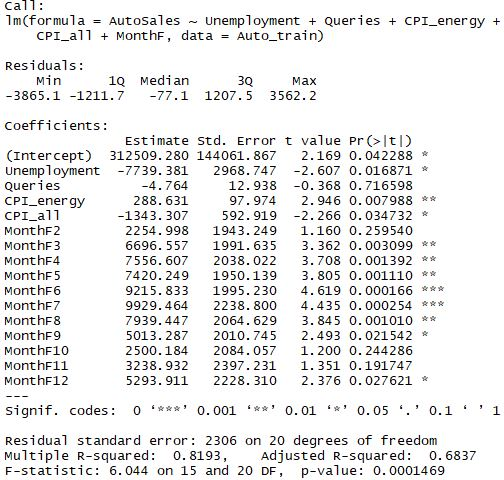
\includegraphics[width=0.36\textheight]{3e.jpg}
  \caption{Question 3(e)}\label{fig:q3.5}
\end{figure}
\textcolor{Blue}{After the looking at the summary of this model (see Figure \ref{fig:q3.5}), we can see that summer, especially June and July, is the peak season for auto sales.}
\\
~
\\
(f) Another peculiar observation about the regression results (with month as a factor variable) is that the signs of the Queries variable and the CPI\_energy variable. Why their signs are counter-intuitive? Please try to give an explanation for such phenomenon and find a way to address this issue. You may need to remove some independent variables and re-build the linear regression model.
\\
\\
\textcolor{Blue}{It seems counter-intuitive that Queries should expect a positive sign and CPI should expect a negative sign but both of them are assigned an opposite sign in the model as expected.
\\
It is a matter of multicolinearity. There are high correlations among Queries, CPI\_all and CPI\_energy.
Therefore, we need a reduced model by removing Queries, which has the highest p-values.}
\textcolor{Blue}{Here we create a new reduced model called AutoLM\_newF\_reduced with removing Queries from the AutoLM\_newF model in (e). Also, after checking the correlation of this model, we find CPI\_energy and CPI\_all are still highly correlated. Therefore, it is better to remove these two variables from the model AutoLM\_newF\_reduced and create another model AutoLM\_newF\_reduced2, which only contains Unemployment and MonthF.
\\
Specifically,
\\
AutoLM\_newF\_reduced = lm(AutoSales $\sim$ Unemployment +  CPI\_energy + CPI\_all + MonthF,  data=Auto\_train)
\\
AutoLM\_newF\_reduced2 = lm(AutoSales $\sim$ Unemployment + MonthF, data=Auto\_train)}
\\
\textcolor{Blue}{We are going to do out-of-sample tests to all the models in (g).}
~
\\
\\
(g) Use out-of-sample test to evaluate all your models built to estimate the sales of Auto. Report the out-of-sample $R^2$ of each model and discuss which model you would like recommend to this Auto Brand for their sales forecasting.
\\
\\
\textcolor{Blue}{In the model AutoLM, out-of-sample $R^2$ = 0.4975116 }
\\
\textcolor{Blue}{In the model AutoLM\_new, out-of-sample $R^2$ = 0.4662344}
\\
\textcolor{Blue}{In the model AutoLM\_newF, out-of-sample $R^2$ = 0.7426902}
\\
\textcolor{Blue}{In the model AutoLM\_newF\_reduced, out-of-sample $R^2$ = 0.7280232}
\\
\textcolor{Blue}{In the model AutoLM\_newF\_reduced2, out-of-sample $R^2$ = 0.8793167}
\\
\textcolor{Blue}{Here we recommend the last model because it 1) has a higher out-of-sample $R^2$ than the other models;  2) it includes Month as factor instead of numeric, which makes the seasonality more interpretable; 3) it has dropped highly correlated variable Queries, CPI\_all and CPI\_energy, which can deal with the problem of multicolinearity.}

\newpage
\noindent\textbf{4. Child IQ}
\\
~
\\
Build a model to predict the IQ of a child based on covariates about his/her mom using the data set \verb+kidiq.csv+. Below are the variables contained therein
\begin{itemize}
	\item $kid\_score$: IQ score of the kid
	\item $mom\_hs$: whether the mom has attained high school (1/0)
	\item $mon\_iq$: mom's IQ score
	\item $mon\_work$: a numerical variable ranges from 1 to 4,
	\begin{itemize}
		\item $1=$did not work in the first three years of the child's life
		\item $2=$worked in the 2nd or 3rd year of child's life
		\item $3=$worked part-time in the first year of child's life
		\item $4=$worked full-time in the first year of child's life
	\end{itemize}
	\item $mom\_age$: age of the mom when delivering the child.
\end{itemize}
Which variables do you recommend to be included into the independent variables? Please report all the steps and results of your analysis. Please also interpret your results.
\\
\textcolor{Blue}{After testing several models, we have decided to choose the following model:
\\
kid\_score =-11.48+51.27 mom\_hs+0.97mom\_iq-0.48mom\_hs*mom\_iq, 
\\
where if mom\_hs = 1, it is associated with 51.27 increase in kid\_score and one unit change in mom\_iq is associate with 0.49 increase in kid\_score;
\\
if mom\_hs = 0, one unit change in mom\_iq is associate with 0.97 increase in kid\_score
\\
Following are the steps and analysis:}
\\
\textcolor{Blue}{1. Plot Scatter between kid\_score and each variable.}
\\
\textcolor{Blue}{2. Split data into training set and testing set
\\
3. Construct model: regress kid\_score on the rest of variables and observe the result.
\\
model1 = lm(kid\_score $\sim$ mom\_hs+mom\_iq+mom\_work+mom\_age , data=kidIQ)
} Figure \ref{fig:q4.1}
\begin{figure}[htbp]
  \centering
  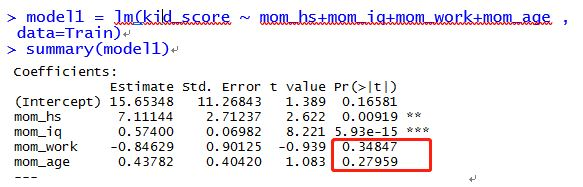
\includegraphics[width=0.6\textheight]{4a.jpg}
  \caption{Question 4(step3)}\label{fig:q4.1}
\end{figure}
\\
\textcolor{Blue}{From above picture, we find that the P-value of the mom work and mom age are greater than 0.05. It implies that mom work and mom age are insignificant variables. We build a new model by drop these two variables.}
\\
\textcolor{Blue}{4. Regress kid\_score on mom\_hs and mom\_iq.
\\
See Figure \ref{fig:q4.2}}
\\
~
\begin{figure}[htbp]
  \centering
  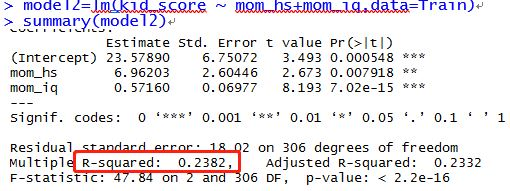
\includegraphics[width=0.4\textheight]{4b.jpg}
  \caption{Question 4(step4)}\label{fig:q4.2}
\end{figure}
\\
\textcolor{Blue}{5. We find variables are significant. Then, we want to improve the R squared. The interaction term is taken into consideration.}
Figure \ref{fig:q4.3}
\\
\\
\begin{figure}[htbp]
  \centering
  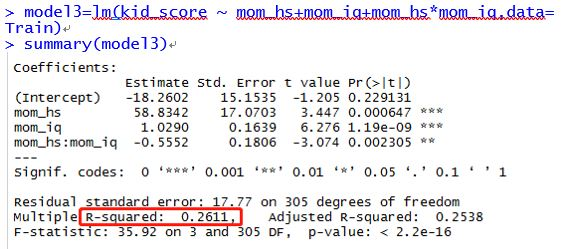
\includegraphics[width=0.4\textheight]{4d.jpg}
  \caption{Question 4(step5)}\label{fig:q4.3}
\end{figure}
~
\textcolor{Blue}{R squared is improved.}
~
\\
\textcolor{Blue}{6. We observed that mom\_work can be regraded as factor variables, then we could construct a new model. See Figure \ref{fig:q4.4}, mom\_work are also not significant variables.}
\begin{figure}[htbp]
  \centering
  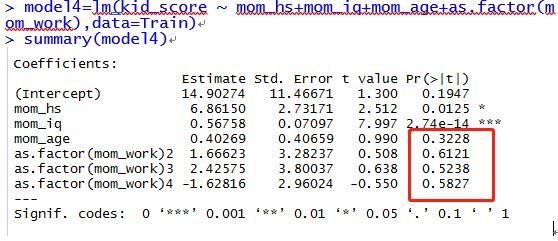
\includegraphics[width=0.4\textheight]{4e.jpg}
  \caption{Question 4(step6)}\label{fig:q4.4}
\end{figure}
\\
\\
\\
\\
\\
\\


\textcolor{Blue}{7. We use testing set to test model2 and model3: See \ref{fig:q4.5}}
\\
\begin{figure}[htbp]
  \centering
  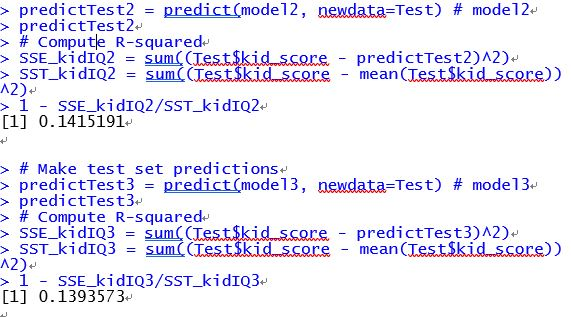
\includegraphics[width=0.4\textheight]{4f.jpg}
  \caption{Question 4(step7)}\label{fig:q4.5}
\end{figure}
\\
~
\textcolor{Blue}{From the test data, we should choose the model:
\\
kid\_score= 23.57890+ 6.96203*mom\_hs+ 0.57160* mom\_iq;
\\
In fact, the difference between model2 and model3 is very small. You also could choose model3.
\\
kid\_score= -18.2602+ 58.8342*mom\_hs+ 1.0290* mom\_iq -0.5552* mom\_hs*mom\_iq.
}


\end{document}
